\chapter{Metodologia}
\label{ch:metodologia}
%Falar porquê do Scrum
%Falar o porquê do Plone

\hspace{2.5cm}

No capítulo de metodologia o objetivo é descrever como ocorreu o processo de construção do sistema, desde a justificativa para a escolha dos métodos de desenvolvimento até a completa entrega do software ao cliente. 

O capítulo está dividido no seguinte escopo: as seções \ref{sec:defMetodologia} e \ref{sec:defCMS}, que justificam a escolha da metodologia e do gerenciador de conteúdo para a implementação do sistema; a seção \ref{sec:desenvolvimento} apresenta como todas as etapas de implementação e reuniões com o cliente foram estabelecidas; e, por último, a seção \ref{sec:testes} aborda como os testes de software foram feitos e o desempenho obtido pela aplicação web.

\hspace{2.5cm}

\section{Definição do tipo de metodologia ágil de desenvolvimento}
\label{sec:defMetodologia}

\hspace{2.5cm}

Vários são os motivos para a escolha do \textit{Scrum} como metodologia de desenvolvimento e \citeonline[~p. 560]{Vasconcelos2015} divulga diversos deles em seu trabalho. A diminuição de reclamações \apud{mann2005case}{Vasconcelos2015}, o aumento do retorno do investimento em projetos de novos produtos \apud{sulaiman2006agileevm}{Vasconcelos2015}, a melhoria da qualidade do produto produzido e diminuição dos custos de produção \apud{sutherland2008fully}{Vasconcelos2015}, e a diminuição no tempo gasto para terminar projetos de desenvolvimento de novos produtos \apud{sanders2007using}{Vasconcelos2015}.

Três características pertencentes ao \textit{Scrum} são a leveza, a simplicidade de entender e a dificuldade de se dominá-lo \apud{sutherland2007scrum}{painka12013utilizaccao}, isto porque é fácil entender suas etapas e o papel de cada um no projeto, mas para adequar essa metodologia à realidade da empresa é necessário experiência e conhecimento.

Assim, às vezes pode ser conveniente alterar prazos, papéis e etapas da metodologia, visando torná-la uma ferramenta de auxílio customizada, e fatores como disponibilidade de clientes, curtos prazos ou complexidade das tarefas devem intervir em decisões dessa espécie, por isso cada projeto utiliza o \textit{Scrum} de uma maneira, ficando a critério das equipes, em especial o \textit{Scrum Master}, quando e onde remodelar.

\hspace{2.5cm}
\subsection{Sobre o \textit{Scrum}}
\hspace{2.5cm}

O \textit{Scrum} é um processo para construção incremental de softwares em ambientes complexos e provê o desenvolvimento de softwares em curtas iterações, denominadas \textit{sprints} \citeonline{rising2000scrum}.

\textit{Sprints}: Cada \textit{sprint} inclui todas as fases de um software modelo de ciclo de vida de desenvolvimento, como design, implementação, testes, revisão de clientes, etc \cite{matharu2015empirical}. Elas têm duração de até 30 dias e também compreendem o procedimento de adaptação a mudança de variáveis (requisitos, tempo, recursos, tecnologia), pois em seu término há sempre uma reflexão sobre as tarefas, definidas antes do início do ciclo, que foram realizadas com sucesso e os próximos incrementos ou revisões as serem executados nas próximas \textit{sprints}, de acordo com o \textit{feedback} passado na reunião com o cliente \citeonline{awad2005comparison}. 

Existem cinco características únicas para o desenvolvimento baseado em \textit{Scrum} \citeonline{matharu2015empirical}, são eles:

\begin{enumerate}
 \item Colaboração: a promoção da colaboração se dá pelo fato do desenvolvimento ser conduzido por equipes compostas por pessoas multifuncionais, envolvendo programadores, arquitetos de software e especialistas em qualidade de software.
 
 \item Encontros diários: são reuniões de curta duração, comandadas pelo \textit{Scrum Master}, onde as equipes de desenvolvimento se comunicam e discutem o progresso com que os requisitos encontrados no \textit{product backlog} estão sendo implementados. \citeonline{rising2000scrum} afirma que esses encontros podem ser realizados três ou quatro vezes na semana e neles os assuntos mais frequentes se baseiam nas dificuldades encontradas e como vencer os obstáculos até a próxima reunião.
 
 \item \textit{Product Backlog}: o \textit{product backlog} captura os requisitos que devem ser entregados, sendo ordenados por nível prioridade. Ele ainda contém erros resolvidos, características gerais e requisitos não funcionais do software.
 
 \item \textit{Sprint Backlog}: este item registra a lista de tarefas que deverão ser realizadas durante a próxima \textit{sprint}. Logicamente a lista de tarefas deve ser baseada no rendimento das equipes, para que não haja um planejamento de quantidade de itens exorbitante que dificilmente serão cumpridos. 
 
 \item Regras: são regras fundamentais da metodologia segundo \citeonline{matharu2015empirical}:
 \begin{itemize}
  \item PO \textit{(Product Owner)}: ``responsável pela definição, priorização e comunicação dos requisitos de produto e guias do processo de desenvolvimento'' \cite[~p. 3, tradução nossa]{matharu2015empirical}.
  
  \item Time de desenvolvimento: equipes compostas de 3 a 9 indivíduos responsáveis por executar as tarefas previstas pelo PO.
 
  \item \textit{Scrum Master}: responsável por guiar as equipes no respeito às regras e princípios do \textit{Scrum}. Ele remove impedimentos e auxilia no processo de desenvolvimento.
  
 \end{itemize}
 
\end{enumerate}


Em pesquisa realizada pelo \textit{State of Agile Report} (Estado de Relatório Rápido, em português), em 2019, 72\% das empresas que participaram responderam praticar com \textit{Scrum} ou uma metodologia híbrida que o utiliza como metodologia de desenvolvimento. Tal pesquisa, encontrada em \cite{relatorioAnual2019}, foi realizada pela décima terceira vez em 2019 e coletou informações sobre metodologias de processos e desenvolvimento de empresas e organizações da Europa, Ásia, América do Sul e África dos mais variados ramos, tais como de tecnologia, de transporte, industrial, governamental e energético.

Os resultados obtidos com a pesquisa identificam a importância de se conhecer a metodologia estudada nesta seção e como ela ainda é usada por empresas do mundo inteiro. Com o objetivo de assegurar e dar ainda mais veracidade a esta conclusão, outra pesquisa, esta realizada em funcionários da empresa de tecnologia \textit{Microsoft} e via web, detalhada em \citeonline{begel2007usage}, aponta que, das 192 respostas recebidas, a maioria das pessoas que trabalham com desenvolvimento, testes e funções de gerenciamento diretamente ligadas a produção de software aplicam o \textit{Scrum} como a metodologia padrão para construir seus produtos, como aponta a figura \ref{ageis-microsoft}. 

\begin{figure}[htb]
 \centering
 \caption{Diferentes metodologias utilizadas pelos funcionários}
 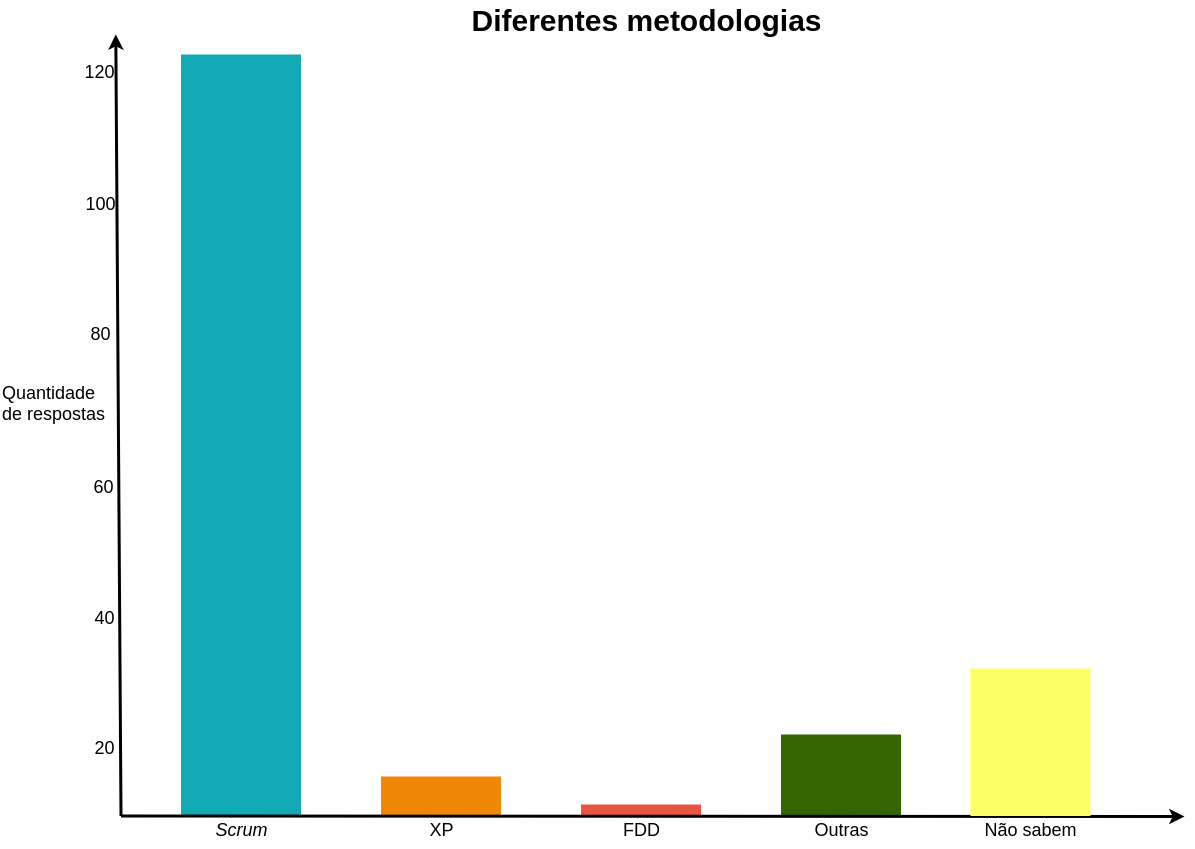
\includegraphics[width=0.8\textwidth]{figuras/diferentes-metodologias}
 \fonte{\citeonline{begel2007usage}. Adaptado.}
 \label{ageis-microsoft}
\end{figure}


\hspace{2.5cm}
\section{Definição do gerenciador de conteúdo}
\label{sec:defCMS}

\hspace{2.5cm}

Analisando as informações extraídas na subseção 2.3.2, no capítulo 2, o gerenciador de conteúdo escolhido pelo autor foi o \textit{Plone}. Os principais fatores que influenciaram nesta decisão estão atrelados ao desempenho e segurança de \textit{websites} construídos com esse CMS. Também é importante destacar que o \textit{Plone} é bastante usado para criação de portais, por exemplo o portal da UFVJM, que possuem características semelhantes ao sistema da Kuruatuba, como a publicação de notícias e eventos. 

O \textit{Plone} possui ferramentas personalizadas e de fácil manipulação que facilitam o gerenciamento de notícias e eventos, primeiramente por possuir campos e opções já pré definidos para o tipo de conteúdo que o usuário irá inserir, e por último por inserir automaticamente o conteúdo criado na lista de conteúdos, devido a uma configuração realizada somente uma vez ao criar o sistema. Sendo assim, basta que o usuário preencha os dados relacionados ao tipo de conteúdo (notícia ou evento) para que ele seja criado e já exibido na página web.

Um dos pontos positivos do \textit{Plone} se consiste, ainda, que sua utilização não necessita da instalação de \textit{plug-ins}, extensões ou complementos, podendo ter seus elementos estáticos, como rodapé e cabeçalho, personalizados via \textit{Portlets}, que segundo \citeonline{UFRGS2012}, são aplicativos e ferramentas prontas para uso em qualquer instalação padrão, podendo ser usadas para calendário, notícias, eventos, menu de busca, enquetes, etc. 

\hspace{2.5cm}

\section{Desenvolvimento}
\label{sec:desenvolvimento}

\hspace{2.5cm}
%Definir as etapas 
%Levantamento de requisitos (histórias de usuário) - construção das sprints - Casos de uso e fluxos alternativos


\subsection{Coleta de requisitos e elaboração de histórias de usuário}

\hspace{2.5cm}

\subsection{Definição das \textit{sprints}}

\hspace{2.5cm}

\subsection{Casos de uso e fluxos alternativos}

\hspace{2.5cm}

\subsection{Apresentação das telas}

\hspace{2.5cm}

\subsection{Estrutura de \textit{containers} do sistema}

\hspace{2.5cm}

Como o sistema deve gerenciar dois tipos de público, um de associados e outro de usuários, resolveu-se criar 3 \textit{containers}: um responsável pelo \textit{Plone} que, por sua vez, apresenta o \textit{website} da Kuruatuba para os visitantes; um \textit{container} responsável por comportar o sistema de gerenciamento de associados, desenvolvido na linguagem PHP, que é conhecida como uma linguagem de programação da era da Web 2.0 que permite o desenvolvimento ágil de software do lado do servidor \citeonline{suzumura2008performance}; e um \textit{container} abrigando o banco de dados, construído com a ferramenta \textit{MySQL}, que possui as informações relacionadas aos associados e onde são realizadas as consultas por parte do sistema escrito em PHP.

O relacionamento dos \textit{containers} acima estão representados na figura  \textbf{colocar aqui a figura dos containers} :


A criação e comunicação dos \textit{containers} compactua com as vantagens descritas na seção 2.6 do capítulo 2, principalmente no que diz respeito à portabilidade e disponibilidade dos recursos. Tais benefícios também se aplicam à segurança, visto que para uma possível invasão ao sistema, é necessário que o invasor conheça o IP e porta de cada \textit{container} e ainda os dados de acesso tanto ao \textit{website} no \textit{Plone} quanto à aplicação destinada a armazenar os dados sobre os associados.   

Outra justificativa para a divisão das aplicações web está na complexidade de manipulação dos SGBDs - Sistema de Gerenciamento de Banco de Dados - não relacionais. Como já explicado na subseção 2.3.1, no capítulo 2, o \textit{Plone} utiliza o banco de dados não relacional \textit{ZODB}, e o mesmo é bastante complexo quando o desenvolvedor necessita realizar consultas ou inserções a seus objetos, sendo inviável a criação de páginas ou elementos para tal tarefa.  

\hspace{2.5cm}
\section{Execução de testes de desempenho}
\label{sec:testes}
\hspace{2.5cm}

